%******************* START ****************************
%\documentclass[12pt,mathdesign]{ndsu-thesis-2022}
\documentclass[12pt,mathdesign,showframe,showgrid]{ndsu-thesis-2022}


%******** Load necessary packages below **********

\title{The NDSU thesis test test test test test test test test test test test test test test test test test test }

%------------------------------------------------------------------
%******************* Document start *******************
\begin{document}
%Barebone - document --- Put your code to test below:


%------------------------------------------------------------------
\myheading{NDSU Grad School Unacceptable Vertical Spacing Around Float Elements}

\section{The NDSU Thesis Vertical Spacing Convention Around Elements}

\textcolor{magenta}{The following figure describes the vertical spacing convention to be followed in the thesis. Each grid represents $0.1 \times 0.1$ inch.} 

\todo{Excess vertical spacing here!}

\myfig[0.0in]{h!}{0.99}{verticalSpacing}{The ``vertical spacing rule'' figure showing different spaing in terms of grid and inch units. Use \texttt{\textbackslash vspace}\{ \ldots \} command with +ve and -ve arguments to correct.}{fig1}

\todo{Excess vertical spacing here! $>$ 3.33 grids}

\kant[9]

%------------------------------------------------------------------
\newpage

\kant[1-2]

\todo{Excess spacing below! $>$ 3.33 grids}

\begin{equation}
P(x) = ax^3+bx^2+cx+d
\end{equation}

\todo{Excess spacing here! $>$ 3.33 grids}

%\kant[3]

\kant[9]

\todo{Less spacing! $<$ 3.33 grids}

\begin{figure}[h!]
\centering
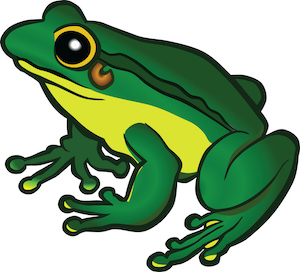
\includegraphics[width=0.6\textwidth]{frog.jpg}
\caption{The green and yellow pet frog - long long long long long long long long caption.}
\end{figure}

\todo{Excess spacing here! Around 3.33 grids} 

\kant[10-11]

\todo[color=green]{Correct spacing here! $>$ 3.33 grids}

\begin{table}[ht]
\centering
\caption{Table spanning entire width (full-width) using \texttt{setlength} and
\texttt{tabcolsep}.}
\vspace{-1ex}
\begin{tblr}{X X[c] X[r] X[r]}
\toprule
Number & Name of month & Days & Season\\
\midrule
\#4 	& April  & 30		& Spring\\
\#5 	& May    & 31		& Summer\\
\#6 	& June   & 30		& Summer\\
\bottomrule
\end{tblr}
\begin{tablenotes}[flushleft]
\item \hspace{-1ex} Note: The \texttt{tablenotes} environment produces table footnotes. 
\end{tablenotes}
\label{tab:2}
\end{table}	

\todo{Excess spacing here!}

\kant[9]

\todo[color=green]{Excess spacing at the page end is OK. As the float on the next page cannot be accommodated here!}


%------------------------------------------------------------------
\newpage
\myfig[0.0in]{h!}{0.9}{frog}{The green and yellow pet frog - long long long long long long long long caption.}{fig1}

\todo{Excess spacing here!}

\kant[9]




%------------------------------------------------------------------
%------------------------------------------------------------------
\myheading{The solution to vertical spacing around float elements using vspace\{ \ldots \} command}

\section{The NDSU Thesis Vertical Spacing Convention Around Elements}

\textcolor{magenta}{The following figure describes the vertical spacing convention to be followed in the thesis.} 

\todo[color=green]{Correct spacing!}

\vspace{-0.2in}%2 grids
\myfig[0.0in]{h!}{0.99}{verticalSpacing}{The ``vertical spacing rule'' figure showing different spaing in terms of grid and inch units. Use \texttt{\textbackslash vspace}\{ \ldots \} command with +ve and -ve arguments to correct.}{fig1}

\todo[color=green]{Correct spacing!}

\vspace{-0.27in}%2.7 grids
\kant[9]

\todo[color=green]{Spacing page end. Okay!}

%------------------------------------------------------------------
\newpage

\kant[1-2]

\todo[color=green]{Correct spacing. Using myeqn shortcut}

\myeqn{% automatic spacing through shortcut
P(x) = ax^3+bx^2+cx+d
}

\todo[color=green]{Correct spacing!}

%\kant[3]

\kant[9]

\todo[color=green]{Correct spacing!}

\vspace{0.1in}%1 grid
\begin{figure}[h!]
\centering
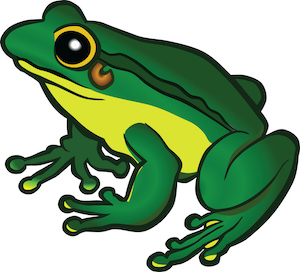
\includegraphics[width=0.6\textwidth]{frog.jpg}
\caption{The green and yellow pet frog - long long long long long long long long caption.}
\end{figure}

\todo[color=green]{Correct spacing!}

\vspace{-0.25in}%2.5 grids
\kant[10-11]

\todo[color=green]{Correct spacing here!}

\begin{table}[ht]
\centering
\caption{Table spanning entire width (full-width) using \texttt{setlength} and
\texttt{tabcolsep}.}
\vspace{-1ex}
\begin{tblr}{X X[c] X[r] X[r]}
\toprule
Number & Name of month & Days & Season\\
\midrule
\#4 	& April  & 30		& Spring\\
\#5 	& May    & 31		& Summer\\
\#6 	& June   & 30		& Summer\\
\bottomrule
\end{tblr}
\begin{tablenotes}[flushleft]
\item \hspace{-1ex} Note: The \texttt{tablenotes} environment produces table footnotes. 
\end{tablenotes}
\label{tab:2}
\end{table}	

\todo[color=green]{Correct spacing!}

\vspace{-0.2in}%2.5 grids
\kant[14]

\todo[color=green]{Excess spacing at the page end is OK. As the float on the next page cannot be accommodated here!}


%------------------------------------------------------------------
\newpage
\myfig[0.0in]{h!}{0.75}{frog}{The green and yellow pet frog - long long long long long long long long caption.}{fig1}

\todo[color=green]{Correct spacing!}

\vspace{-0.2in}%2.5 grids
\kant[9]

\textcolor{magenta}{\emph{Note}: Compare the source code of chapters 1 and 2 to understand how the spacing is adjusted. Once done activate line 2 and comment to see the final output. Of course, this can be done at any time during development as well. Needless to say the \texttt{todo} commands can be removed. Also, understand that whatever spacing given by \LaTeX{} is actually correct but we make these adjustments to comply with the NDSU-approved thesis format.}


\end{document}
%******************* END *******************************